\documentclass[border=5pt]{standalone}
\usepackage{tikz}
\usepackage{amsmath}
\usetikzlibrary{positioning, arrows.meta, calc, fit, backgrounds, shapes.geometric}

% --- Color Scheme (Blue-Gray) ---
\definecolor{bgPrimary}{HTML}{DAE8FC}
\definecolor{bgSecondary}{HTML}{E8EEF7}
\definecolor{bgAccent}{HTML}{B3CDE3}
\definecolor{bgInput}{HTML}{F0F4F8}
\definecolor{borderPrimary}{HTML}{6C8EBF}
\definecolor{borderAccent}{HTML}{3A6EA5}
\definecolor{arrowColor}{HTML}{4A6A8A}
\definecolor{textMain}{HTML}{2C3E50}
\definecolor{textLight}{HTML}{7F8C8D}
\definecolor{bgHighlight}{HTML}{FFF3CD}
% Canary-specific colors
\definecolor{bgGreen}{HTML}{D5F5E3}
\definecolor{borderGreen}{HTML}{27AE60}
\definecolor{bgOrange}{HTML}{FDEBD0}
\definecolor{borderOrange}{HTML}{E67E22}
\definecolor{bgRed}{HTML}{FADBD8}
\definecolor{borderRed}{HTML}{E74C3C}

% --- Styles ---
\tikzset{
  module/.style={draw=borderPrimary, fill=bgPrimary, rounded corners=4pt,
    minimum width=2.8cm, minimum height=1.2cm,
    font=\sffamily\small, text=textMain, line width=0.6pt, align=center},
  novelmodule/.style={draw=borderAccent, fill=bgAccent, rounded corners=4pt,
    minimum width=2.8cm, minimum height=1.2cm,
    font=\sffamily\small\bfseries, text=textMain, line width=1.0pt, align=center},
  iobox/.style={draw=borderPrimary, fill=bgInput, rounded corners=3pt,
    minimum width=2cm, minimum height=1cm,
    font=\sffamily\small, text=textMain, line width=0.5pt, align=center},
  stdarrow/.style={-{Stealth[length=5pt, width=4pt]}, line width=0.6pt, color=arrowColor},
  branchbox/.style={rounded corners=4pt, minimum width=3.0cm, minimum height=0.8cm,
    font=\sffamily\small\bfseries, text=textMain, line width=0.8pt, align=center},
  userbox/.style={draw=borderPrimary, fill=bgInput, rounded corners=2pt,
    minimum width=0.6cm, minimum height=0.5cm,
    font=\sffamily\tiny, text=textMain, line width=0.4pt, align=center},
  scorebox/.style={draw=borderPrimary, fill=bgSecondary, rounded corners=3pt,
    minimum width=2.4cm, minimum height=0.7cm,
    font=\sffamily\scriptsize, text=textMain, line width=0.5pt, align=center},
  decision/.style={diamond, draw=borderAccent, fill=bgHighlight,
    minimum width=1.6cm, minimum height=1.2cm,
    font=\sffamily\scriptsize\bfseries, text=textMain, line width=0.8pt,
    align=center, inner sep=2pt, aspect=2},
  outgreen/.style={draw=borderGreen, fill=bgGreen, rounded corners=3pt,
    minimum width=2.0cm, minimum height=0.7cm,
    font=\sffamily\small\bfseries, text=textMain, line width=0.8pt, align=center},
  outred/.style={draw=borderRed, fill=bgRed, rounded corners=3pt,
    minimum width=2.0cm, minimum height=0.7cm,
    font=\sffamily\small\bfseries, text=textMain, line width=0.8pt, align=center},
}

\begin{document}
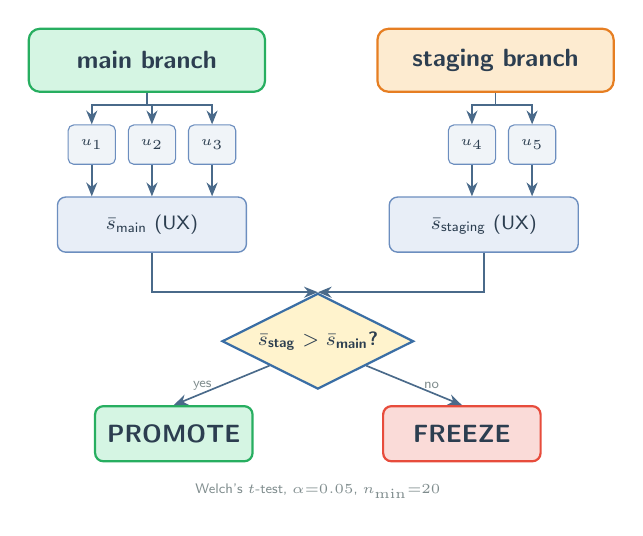
\begin{tikzpicture}

  % === Row 1: Two branches side by side ===
  \node[branchbox, draw=borderGreen, fill=bgGreen] (mainbr) {main branch};
  \node[branchbox, draw=borderOrange, fill=bgOrange, right=1.4cm of mainbr] (stagbr) {staging branch};

  % === Row 2: Users under each branch ===
  \node[userbox, below=0.4cm of mainbr, xshift=-0.7cm] (u1) {$u_1$};
  \node[userbox, right=0.15cm of u1] (u2) {$u_2$};
  \node[userbox, right=0.15cm of u2] (u3) {$u_3$};

  \node[userbox, below=0.4cm of stagbr, xshift=-0.3cm] (u4) {$u_4$};
  \node[userbox, right=0.15cm of u4] (u5) {$u_5$};

  % Arrows: branch -> users
  \draw[stdarrow] (mainbr.south) -- ++(0,-0.15) -| (u1.north);
  \draw[stdarrow] (mainbr.south) -- ++(0,-0.15) -| (u2.north);
  \draw[stdarrow] (mainbr.south) -- ++(0,-0.15) -| (u3.north);
  \draw[stdarrow] (stagbr.south) -- ++(0,-0.15) -| (u4.north);
  \draw[stdarrow] (stagbr.south) -- ++(0,-0.15) -| (u5.north);

  % === Row 3: Score boxes ===
  \node[scorebox, below=0.4cm of u2] (smain) {$\bar{s}_{\text{main}}$ (UX)};
  \node[scorebox, below=0.4cm of u4, xshift=0.15cm] (sstag) {$\bar{s}_{\text{staging}}$ (UX)};

  % Arrows: users -> scores
  \draw[stdarrow] (u1.south) -- (u1.south |- smain.north);
  \draw[stdarrow] (u2.south) -- (smain.north);
  \draw[stdarrow] (u3.south) -- (u3.south |- smain.north);
  \draw[stdarrow] (u4.south) -- (u4.south |- sstag.north);
  \draw[stdarrow] (u5.south) -- (u5.south |- sstag.north);

  % === Row 4: Decision diamond ===
  \coordinate (scoreMid) at ($(smain.south)!0.5!(sstag.south)$);
  \node[decision, below=0.5cm of scoreMid] (dec) {$\bar{s}_{\text{stag}} > \bar{s}_{\text{main}}$?};

  % Arrows: scores -> decision
  \draw[stdarrow] (smain.south) -- (smain.south |- dec.north) -- (dec.north);
  \draw[stdarrow] (sstag.south) -- (sstag.south |- dec.north) -- (dec.north);

  % === Row 5: Outcomes ===
  \node[outgreen, below left=0.5cm and 0.2cm of dec] (promote) {PROMOTE};
  \node[outred, below right=0.5cm and 0.2cm of dec] (freeze) {FREEZE};

  % Arrows: decision -> outcomes
  \draw[stdarrow] (dec.south west) -- node[left, font=\sffamily\tiny, text=textLight] {yes} (promote.north);
  \draw[stdarrow] (dec.south east) -- node[right, font=\sffamily\tiny, text=textLight] {no} (freeze.north);

  % === Statistical annotation ===
  \node[font=\sffamily\tiny, text=textLight, anchor=north] at ([yshift=-0.15cm]$(promote.south)!0.5!(freeze.south)$) {%
    Welch's $t$-test, $\alpha{=}0.05$, $n_{\min}{=}20$};

\end{tikzpicture}
\end{document}
